\chapter{\label{chap:ai}Algoritmos de Inteligência Artificial para Elevadores}

Neste capítulo vamos apresentar:

\begin{itemize}
\item Os detalhes dos algoritmos selecionados e justificar a suas escolhas perante o problema;
\item Introduzir o modelo de simulação do sistema~-~ou seja, a modelagem
prédio/andares/elevadores (e não a modelagem do simulador propriamente dito);
\item Detalhes de cada algoritmo e descrever como esperamos que seja o resultado de seu uso junto ao sistema.
\end{itemize}

A busca pela solução do problema de atribuir elevadores para atender chamadas
feitas pelos passageiros, minimizando alguma métrica, é apresentada pela
literatura pesquisada na forma de alguns algoritmos~\cite{KOEHLEROTTIGER02}.
Tais algoritmos possuem complexidades distintas, indo desde algoritmos triviais,
que sequer podem ser classificados como algoritmos de Inteligência Artificial~-~mas ainda
interessantes para fins de comparação~-~, até soluções mais complexas, onde mais
dados são utilizados de modo a tomar decisões mais complexas.

Em um hipotético cenário ideal, ter-se-ia todos os dados de cada passageiro~-~\textit{i.e.} cada
pessoa que chegasse ao elevador informaria de antemão para qual andar deseja ir.
No entanto, isto não é realista no contexto dos sistemas de elevadores
instalados atualmente, onde cada pessoa apenas informa se deseja subir ou descer. Portanto, os algoritmos
aqui descritos tentam fazer inferências\footnote{\textit{e.g.} Podemos estimar a
lotação do elevador com base no peso reportado pela balança interna do elevador, que já se
  encontra nele por motivos de segurança.} a respeito de dados que não possuem,
quando relevante, ou tentam tomar decisões ignorando os dados que não estão disponíveis.

A seguir descreveremos, do mais simples ao mais complexo, os algoritmos
selecionados para o desenvolvimento na segunda etapa deste trabalho.

\section{\label{sec:ai:nn}Nearest Neighbour}

O algoritmo de \textit{Nearest Neighbour} é o mais ingênuo de todos, e servirá
de base para a avaliação dos demais algoritmos.

Seu funcionamento é trivial: o elevador mais próximo do chamado sempre
atenderá este chamado~\cite{Friese20061908}.

Um dos problemas deste algoritmo é que ele pode causar muitas mudanças de
direção de um elevador, o que acarreta um tempo de espera maior para os
passageiros que estão dentro dele.

Considere, por exemplo, o cenário da Figura~\ref{fig:elevadores:nn:bad}.

\begin{figure}[htb!]
  \centering
  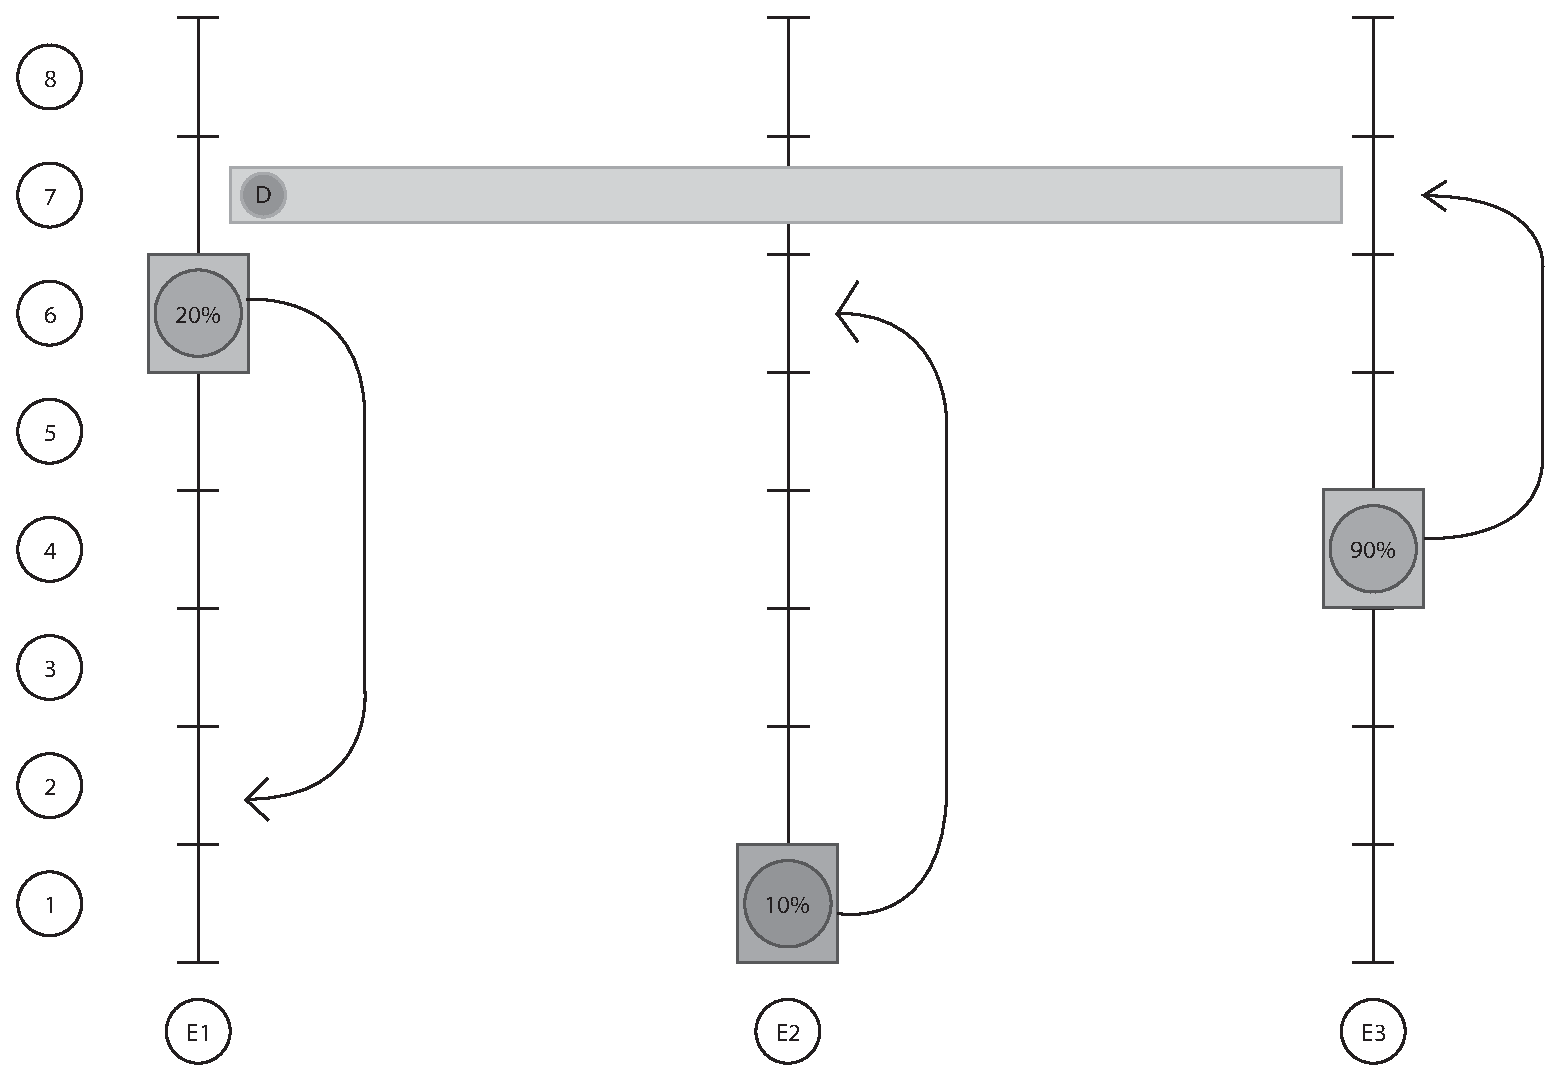
\includegraphics[scale=0.6]{img/elevator_example_nn_bad.eps}
  \caption{Exemplo de sistema de 3 elevadores com 8 andares}
\label{fig:elevadores:nn:bad}
\end{figure}

Caso o algoritmo de \textit{Nearest Neighbour} seja utilizado, o elevador $E1$
seria selecionado para atender o pedido no sétimo andar. Isto é claramente ruim
para os passageiros deste elevador. Além disto, é possível notar que o elevador
$E3$ já tinha uma parada programada no sétimo andar e seria possível atender
este pedido sem alterar a agenda de nenhum elevador. O algoritmo de
\textit{Nearest Neighbour}, no entanto, não leva em consideração estas informações.

O único propósito deste algoritmo é servir de base de comparação com outros
algoritmos propostos, de modo a validarmos o simulador. Espera-se que uma
melhora clara de desempenho seja notada ao comparar-se este com o próximo dos
mais triviais, o \textit{Nearest Neighbour Melhorado}.

\section{\label{sec:ai:nnm}Nearest Neighbour Melhorado}

Uma melhoria que pode ser feita ao algoritmo de \textit{Nearest Neighbour}
é considerar o sentido em que o elevador está indo para atender o
chamado~\cite{Friese20061908}. Isto implica em considerar-se agora
a informação de sentido dos pedidos. É importante notar que ainda não se
considera quantas pessoas fizeram um pedido~-~apenas sabe-se que há pedidos no
andar, e como destinos tem-se ``para cima'', ``para baixo'' ou ambos.

Este algoritmo resolve o problema de mudanças de direção que o algoritmo de
\textit{Nearest Neighbour} sofre.

Considere, novamente, o caso da Figura~\ref{fig:elevadores:nn:bad}. Este
algoritmo considerará apenas os elevadores que estão parados ou indo no sentido
de onde o pedido se encontra. Neste caso, apenas os elevadores $E2$ e $E3$ serão
considerados. O elevador $E3$ está mais próximo do pedido, então será escolhido.

No entanto, sua escolha para este trabalho também se dá para fim de comparação
com os outros e validação do simulador. Como seu comportamento é diferente do
caso mais trivial, mas ainda assim bastante simples, poderá ser visto com clareza
algum tipo de melhora no tempo de resposta do sistema simulado, bem como a validade do simulador.

\section{\label{sec:ai:minimize-cost-function}Minimização da Função de Custo}

O primeiro algoritmo de IA a ser testado é simples: define-se uma
função de custo, inerente a cada elevador, que descreve quão custoso
é atender um pedido, comparado a não atendê-lo~\cite{Friese20061908}.
A decisão de qual elevador é escolhido para atender o pedido é feita com base
em qual deles terá o menor valor da função de custo.

Um exemplo de função de custo é:

\[
  J(e, l, p) = \lambda l(p - e)
\]

Onde:
\begin{itemize}
\item \textbf{$e$} é o número do andar onde o elevador se encontra
\item \textbf{$l$} é o percentual de lotação do elevador
\item \textbf{$p$} é o número do andar onde o pedido se encontra
\item \textbf{$\lambda$} é
  \begin{list}{$\circ$}{}
    \item zero, caso o programa atual do elevador faça com que ele passe por
      aquele andar
    \item $1$, caso o elevador não tenha um programa (\textit{i.e.},
      ele esteja ocioso) ou o elevador esteja indo na direção do pedido.
    \item $2$ caso ele mude de direção para atender este pedido.\footnote{Multiplica-se
        a distância por dois pois é necessário ir até o andar do pedido e então
        voltar para o andar onde se estava anteriormente, para só então atender
        o pedido.}
  \end{list}
\end{itemize}

\begin{figure}[htb!]
  \centering
  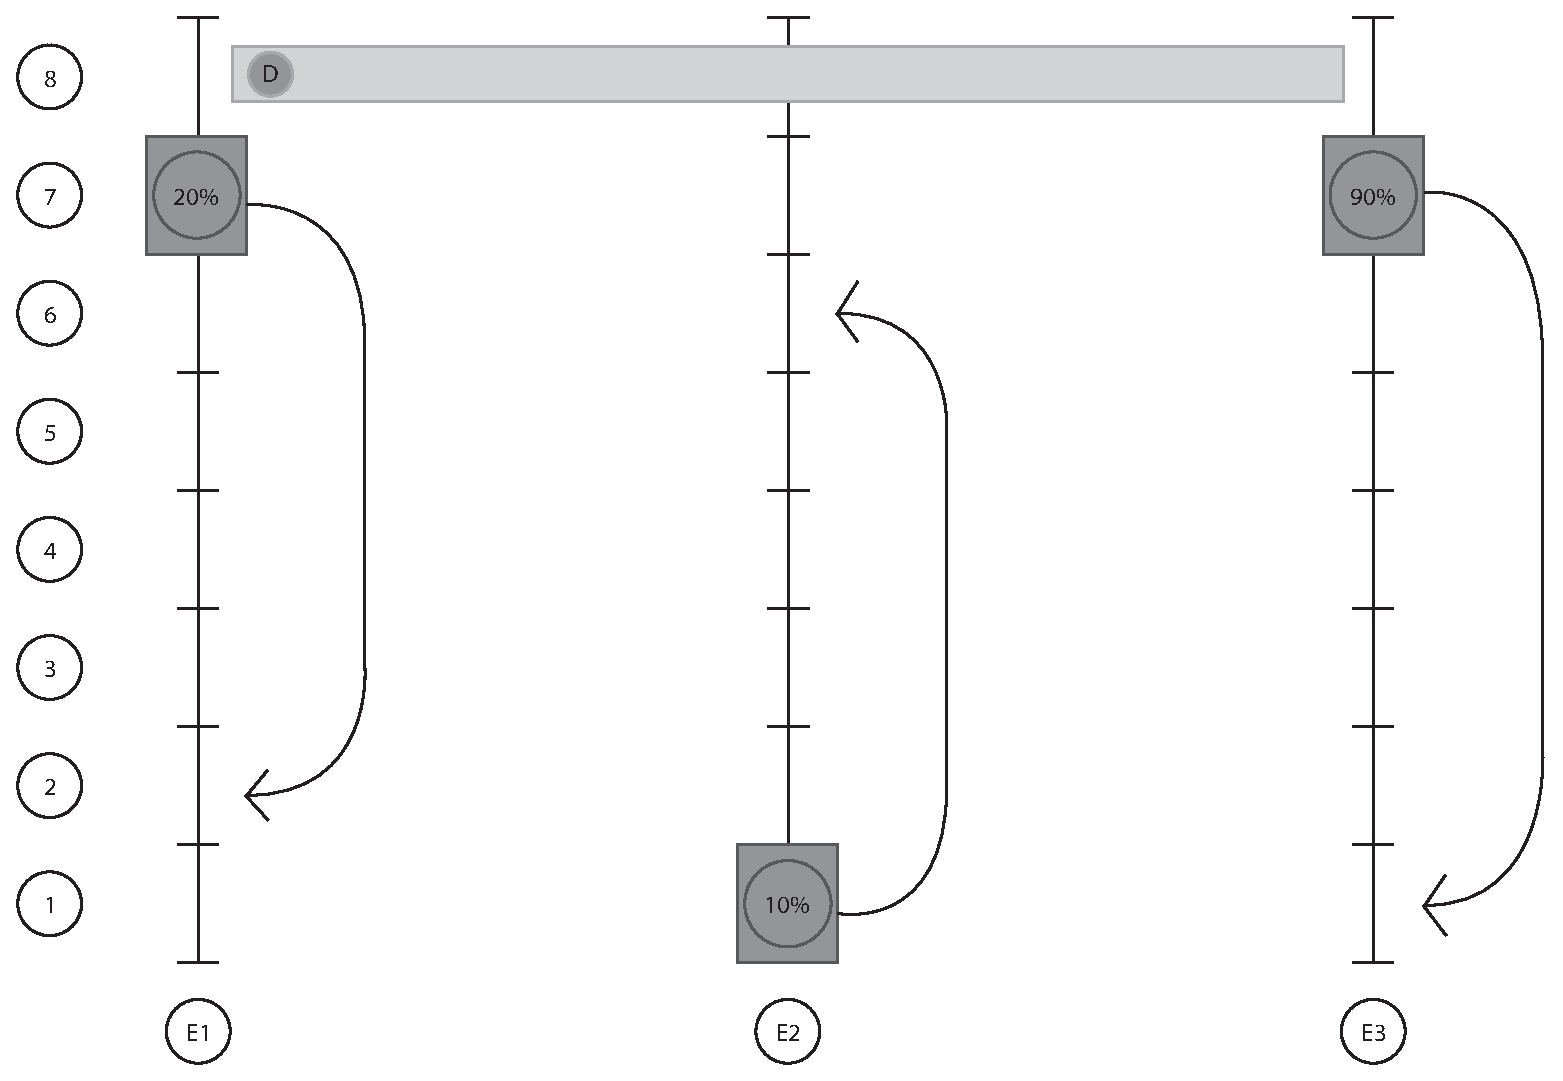
\includegraphics[scale=0.6]{img/elevator_example1.eps}
  \caption[Exemplo de sistema de 3 elevadores com 8 andares]{Exemplo de sistema
    de 3 elevadores com 8 andares, com um pedido para descer a partir do oitavo
    andar. A lotação dos elevadores está representada em percentual dentro
    deles, e seus programas são representados por setas.}
  \label{fig:elevadores-1}
\end{figure}

Utilizando o exemplo da Figura~\ref{fig:elevadores-1}, podemos calcular o custo
de cada elevador. Nela, temos 3 elevadores:

\begin{itemize}
\item \textbf{$E_{1}$} no sétimo andar, com carga $20\%$ e um destino: o segundo andar;
\item \textbf{$E_{2}$} no primeiro andar, com carga $10\%$ e um destino: o sexto andar;
\item \textbf{$E_{3}$} no sétimo andar, com carga $90\%$ e um destino: o primeiro andar;
\end{itemize}

Sabemos que há um pedido no oitavo andar, para descer\footnote{Na
  Figura~\ref{fig:elevadores-1}, representado pelo círculo com um \textbf{D}, de
\textit{Down}.}.

Para o Elevador $E_{1}$:

\[J(7, 0.2, 8) = 2 \times 0.2(8 - 7) = 0.4\]

Neste caso, $\lambda$ é 2, pois o elevador deverá mudar de sentido
(\textit{i.e.}, ele deverá subir até o oitavo andar e então voltar para o sétimo
andar, o que representa um deslocamento de dois andares).

Para o Elevador $E_{2}$:

\[J(1, 0.1, 8) = 1 \times 0.1(8 - 1) = 0.7\]

Neste caso $l$ é $0.1$, pois sua lotação é $10\%$\footnote{Como não temos informações a
respeito do futuro, não podemos considerar alterações na carga de um elevador.},
e $p - e$ é $7$, pois o elevador deverá subir sete andares.\footnote{Pela regra
de cálculo, consideramos apenas a posição atual do elevador, e não a posição que
ele estará ao fim de sua última atividade. Seria possivel alterar esta regra,
gerando uma função de custo levemente diferente, com resultados diferentes. É um
teste válido para a implementação.}

Para o Elevador $E_{3}$:

\[J(7, 0.9, 8) = 2 \times 0.9(8 - 7) = 1.8\]

Neste caso $l$ é $0.9$, pois sua lotação é $90\%$, e $\lambda$ é $2$, pois o elevador
$E_{3}$ deve subir do sétimo para o oitavo andar e descer novamente até o sétimo.

Vemos que, para esta função de custo, neste sistema, é vantajoso mudar o sentido
de $E_{1}$ para atender o chamado no oitavo andar, e depois continuar na direção original.

Várias funções de custo podem ser experimentadas e comparadas: outras funções de
custo levariam em consideração mudanças de direção de viagem
\footnote{\textit{e.g.}, pode ser vantajoso um elevador mudar de direção para
  atender um pedido a um andar de distância, caso a alternativa seja fazer o
  pedido esperar um deslocamendo de dezenas de andares de outro elevador.}, ou
ainda tentar manter todos os custos o mais baixo possível, ao mesmo tempo que o
mais próximos uns dos outros.

Uma outra função de custo possível seria:

\[J(e, l, p) = l(\lambda(p - e))^{2}\]

Esta função penaliza mais o movimento, elevando-o ao quadrado.

Para o exemplo da Figura~\ref{fig:elevadores-1}, temos:

\[J(7, 0.2, 8) = 0.2(2 \times (8-7))^2 = 0.8\]
\[J(1, 0.1, 8) = 0.1(1 \times (8-1))^2 = 6.4\]
\[J(7, 0.9, 8) = 0.9(2 \times (8-7))^2 = 3.6\]

Novamente, para esta função, o Elevador $E_{1}$ é eleito para atender o pedido.

\subsection{Algoritmo}

O Algoritmo~\ref{alg:cost-function} ilustra um algoritmo com o comportamento desta
função.

\begin{algorithm}[htb]
\begin{center}
\begin{algorithmic}[1]
\Function{ChooseElevator}{$call, elevatorSet, costFunction$}
  \State $selectedElevator \leftarrow null$
  \State $minCost \leftarrow \infty$
  \For{\textbf{each} $elevator$ in $elevatorSet$}
    \State $cost \leftarrow \Call{CostFunction}{$call, elevatorSet$}$
    \If{$cost = 0$}
      \State \textbf{return} $elevator$
    \EndIf
    \If{$cost < minCost$}
      \State $selectedElevator \leftarrow elevator$
      \State $minCost \leftarrow cost$
    \EndIf
  \EndFor
  \State \textbf{return} $selectedElevator$
\EndFunction
\end{algorithmic}
\end{center}
\caption
   {\label{alg:cost-function}Função de Custo}
\end{algorithm}

Os argumentos para este algoritmo são:

\begin{description}[leftmargin=!,labelwidth=\widthof{\bfseries $costFunction$}]
  \item[$call$] Abstração de uma chamada;
  \item[$elevatorset$] Conjunto de todos os elevadores do prédio;
  \item[$costFunction$] Ponteiro para a função de cálculo de custo.
\end{description}

Seu funcionamento pode ser descrito como: dada uma chamada, para cada elevador
presente no conjunto calcula-se o retorno da função de custo e o algoritmo
retorna o elevador com a menor função de custo correspondente. Além disso, há
uma otimização (programação dinâmica): se algum elevador possuir custo zero, o
algoritmo retorna imediatamente, como resultado, este elevador - pois nenhum
outro elevador poderá ter um retorno da função de custo melhor do que zero.

\subsection{Nearest Neighbour como Função de Custo}

É possível definir o algoritmo de \textit{Nearest Neighbour} (apresentado na
Seção~\ref{sec:ai:nn}) como uma função de
custo:

\[J(e, p) = p - e\]

Onde considera-se apenas $p - e$, que é a distância entre a posição atual do
elevador ($e$) e o número do andar onde o pedido se encontra ($p$).

\section{Planning}

% TODO: essa explicação pode melhorar ainda

A idéia do algoritmo de planning é estender o de função de custo, calculando-a
para vários passos no futuro~\cite{Koehler00elevatorcontrol}~-~como em um jogo de xadrez. Busca-se o
caminho cuja soma tem o menor custo total depois de vários passos.

Há duas alternativas para esta árvore de decisões: a decisão pode ser ``qual
elevador deve atender o próximo pedido'' (Figura~\ref{fig:planning}),
ou ``qual pedido deve ser atendido por qual elevador''. % TODO: Esta ilustração

O horizonte de cálculo deve ser selecionado, dado que é um fator limitante no
tamanho do cálculo do algoritmo.

Cada decisão diferente, para cada elevador, é um nodo novo na árvore. Ao
escolher-se uma das alternativas (\textit{i.e.} a que, ao final de $x$ eventos
no futuro tem a menor soma de custos), avança-se um passo na simulação e executa-se o
algoritmo novamente.

Na Figura~\ref{fig:planning}, vemos um exemplo hipotético de planning sendo executado com
horizonte 3 e dois elevadores. Para cada passo do algoritmo, a decisão a ser
tomada é ``qual elevador deve atender o próximo pedido da fila?'', e, para isto,
calcula-se a função de custo. O resultado da função pode ser visto entre
parênteses em cada nodo da árvore da Figura~\ref{fig:planning}.

Ao encontrarmos o horizonte (no caso da Figura~\ref{fig:planning}, no nível 3 da
árvore), soma-se os custos até lá (na Figura~\ref{fig:planning}, os círculos
abaixo do nível mais baixo indicam a soma dos custos). O caminho que leva ao
menor custo total é o que deve ser tomado. No exemplo da Figura~\ref{fig:planning}, o
elevador $E2$ atenderá o primeiro e o segundo chamados da fila, e então o
elevador $E1$ atenderá o terceiro chamado, como pode ser visto pelo caminho destacado.

\begin{figure}[htb!]
  \centering
  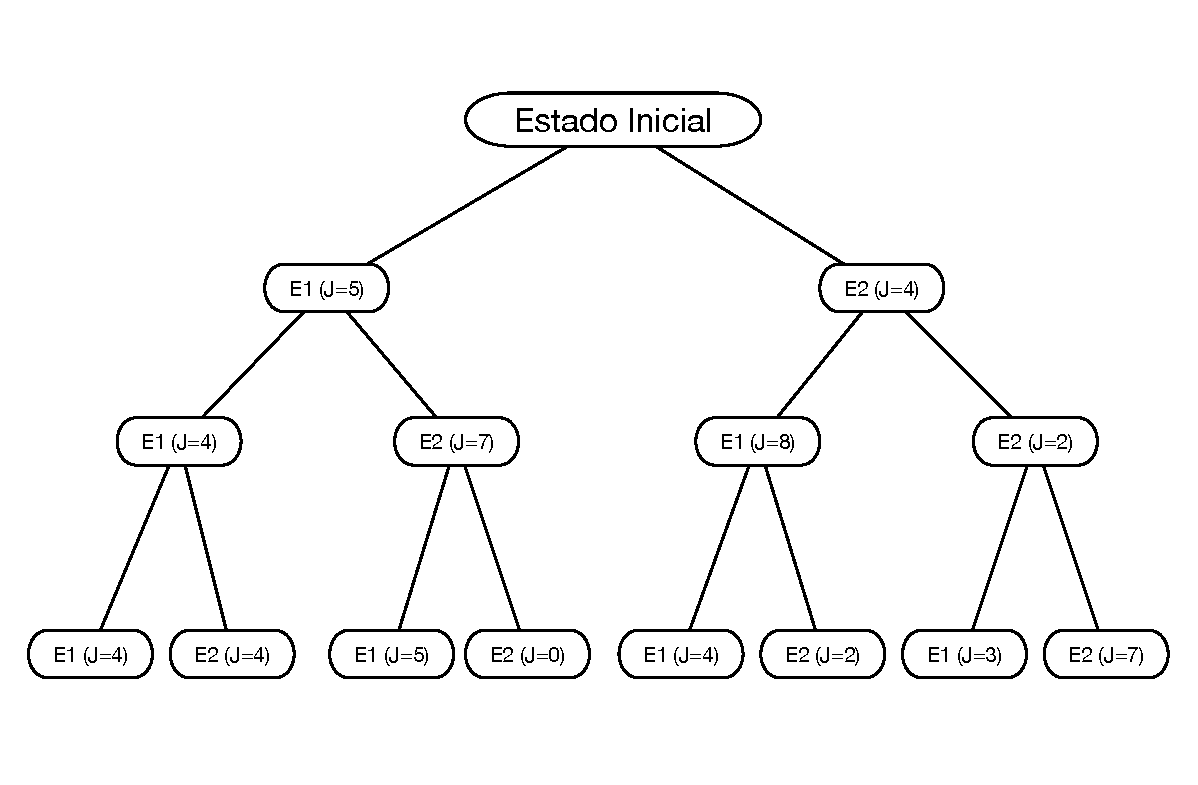
\includegraphics[scale=0.6]{img/planning.eps}
  \caption{Exemplo de planning com horizonte 3 e dois elevadores}
\label{fig:planning}
\end{figure}

O algoritmo é executado (acarretando uma reavaliação) a cada evento do sistema
de simulação, descrito no Capítulo~\ref{chap:modeling}.

\subsection{Função de Custo como Algoritmo de Planning}

Podemos ver que, para cada etapa do algoritmo de planning, estamos avaliando uma
função de custo. Isto fica mais explícito na Figura~\ref{fig:planning}. Se
considerarmos o caso especial de horizonte 1, o resultado do algoritmo seria
idêntico ao de apenas avaliar a função de custo para uma única tomada de
decisão, como proposto na Seção~\ref{sec:ai:minimize-cost-function}.

\section{Planning Multi-Agente}

Este algoritmo é uma extensão do algoritmo de Planning, onde, em vez de termos
um processamento central que decide que um elevador deve atender o pedido, temos
todos os elevadores calculando por conta própria se vale a pena atender um
pedido ou não.

A literatura neste tópico é ainda escassa. Um estudo deste tipo de
comportamento seria interessante, mas dado o tempo disponível para a
implementação e teste, possivelmente não será viável.

Uma possível implementação deste tipo de algoritmo faria com que cada elevador
avaliasse qual pedido, dentre os disponíveis, ele tomaria para si. Para evitar
que todos cheguem à mesma decisão, políticas de escalonamento podem ser
escolhidas. Por exemplo, coloca-se os elevadores em uma fila circular. O
primeiro elevador da fila roda seu algoritmo e calcula qual pedido deve tomar
para si. Ele vai, então, para o fim desta fila, e o próximo elevador toma a
próxima decisão.

Os algoritmos que cada elevador pode utilizar são as variações de funções de
custo e planning, com variações no horizonte.

\section{Políticas de Ociosidade}

Há ainda um outro detalhe a ser considerado, que pode afetar o desempenho do
sistema: o que um elevador deve fazer quando não há chamados para ele.

Há várias possibilidades para isto, e é interessante testar-se várias delas e
comparar-se sua eficácia.

Por exemplo, uma política ingênua seria manter o elevador no último andar onde
ele parou. Outra política, também bastante simples, seria mandar todo elevador
ocioso de volta para o térreo.

Políticas mais inteligentes podem maximizar a distância entre elevadores
ociosos. Por exemplo, o primeiro elevador ocioso deve ir para o térreo. O
segundo, para o andar mais alto. O terceiro, para um andar intermediário~-~e
assim por diante.

Há ainda a possibilidade de analisar-se os padrões de tráfego. Como sabe-se o
histórico de chegadas de passageiros em cada andar, pode ser tomada a decisão de
mandar elevadores ociosos para os andares onde é mais provável que algum novo
pedido surja. No entanto, este tipo de comportamento está fora do escopo deste
trabalho, por motivos de falta de tempo.